%% BEGIN semsamp2.tex
% This is a sample document for seminar.sty, v0.93 (and maybe later).
%
% This file contains both landscape and portrait mode slides.
% Choose one of the following to print them out:
%  - If using PSTricks, try the semcolor style option.
%  - If using Rokicki's dvips, try the semrot style option.
%  - To print the landscape slides, put \landscapeonly in the preamble.
%    To print the portrait slides, include the portrait style option and
%    put \portraitonly in the preamble.
%
%
\documentclass[%
%rrrrrrrrrrrrrrrr\documentstyle[%
  slidesonly,%  Try notes or notesonly instead.
  %10pt,%notes,%      Use instead of slidesonly to typeset the notes.
  %notesonly,%  Use instead of slidesonly to typeset notes and slides.
  %semcolor,%   Try me if using PSTricks.
  %semrot,%     Try me if using Rokicki's dvips.
  %semhelv,%    Try me if using a PostScript printer.
  %article,%    Try me.
  %portrait,%   Try me.
  %sem-a4,%     Try me if using A4 paper.
  semlayer%     This must be included, but you need the semcolor option to
  ]{xseminar}                                  % actually see the overlays.

\slidesmag{5}
\articlemag{1}

%\twoup                     % Try me for twoup printing.

%\portraitonly              % To print only portrait slides
%\landscapeonly             % To print only landscape slides

%\notslides{\ref{questions}-7,1}   %Try me: The slides are omitted.
%\onlyslides{\ref{questions}-7,1}  %Try me: Only these slides are included.
%\onlynotestoo                     %Try me: For selecting notes as well.

\colorlayers{red,blue}      % Try deleting this if using the semcolor option,
                            % to get \blue and \red to use PostScript color.

%\overlaysfalse             % Suppress overlays with semcolor option.
%\layersfalse               % Suppress color layers with semcolor option.

\rotateheaderstrue          % Try this out if using rotation macros.

\usepackage{hyperref}
\usepackage{url}
\usepackage{amsmath}
\usepackage{amsthm}
\usepackage{graphicx}
% \usepackage[pdftex]{graphicx}
\usepackage{amsfonts}
\usepackage{mathrsfs}
\usepackage{amssymb}
\usepackage[noend]{algorithmic}
\usepackage[plain]{algorithm}

\usepackage{color}
\usepackage{ulem}

%\newtheorem{theorem}{Theorem}[section]
\newtheorem{theorem}{Theorem}
\newtheorem{corollary}{Corollary}[section]
\newtheorem{lemma}{Lemma}[section]
\newtheorem{definition}{Definition}[section]
\newtheorem{proposition}{Proposition}[section]
\newtheorem{claim}{Claim}[section]
\newtheorem{model}{Model}[section]
\newtheorem{example}{Example}[section]
%\newtheorem{algorithm}{Algorithm}[section]
%\newenvironment{proof}{\noindent{\bf Proof.}}{\hspace*{\fill} $\Box$}
%\newenvironment{defn}{\noindent \underline{\hspace{7in}}\\ \noindent{\bf Defn:}}{\hspace*{\fill} \newline\noindent\underline{\hspace{7in}}}
\newenvironment{defn}{\noindent \\ \noindent{\bf Defn:}}{\hspace*{\fill} \newline}
\newcommand{\fns}{\footnotesize}
\newenvironment{thm}{\noindent{\bf Theorem:}}{\hspace*{\fill} }
\newcommand{\bare}{\noindent \underline{\hspace{7in}}\\ }
%\newcommand{\myws}{\textcolor{white}{ XXXXXX}}
\newcommand{\vt}{

\vspace{.15in} 

\noindent}

\newcommand{\nvt}{

\vspace{-.15in} 

\noindent}
%\newenvironment{thm}{\noindent{\bf Theorem:}}{\hspace*{\fill} }
%\newcommand{\bare}{\noindent \underline{\hspace{7in}}\\ }
%\newcommand{\myws}{\textcolor{white}{ XXXXXX}}
%\newcommand{\mybul}{{\textcolor{white}{XX}}$\bullet$ }
\newcommand{\myar}{\textcolor{red}{ ==$>$}}
\newcommand{\mybl}{{\textcolor{white}{XX}}{\bf *}}
\newcommand{\n}{\noindent }

\newcommand{\mylg}{\mbox{ lg } }



\newcommand{\tht}{\hspace{.15in} }

\newcommand{\Half}{\mbox{\bf Half}}
\newcommand{\Solve}{\mbox{\bf Solve}}
\newcommand{\Halfc}{\underline{\mbox{\bf Half}}}
\def\4halftbs{XXX\=XXXX\=XXXX\=mmm\kill}

\def\tbs{XXXXXXX\=XXXXX\= \kill}
\def\otbs{XXXXXXX\=XXXXX\=XXX\=XXX\= \kill}
\def\sqrotbs{xxx\=xxx\=xx\kill}
\def\lsqrotbs{xxx\=xxx\=xxx\=xxBBBBBBBBBBBBBBBBBBBBBBBBBBBB\=xxx\=lxx\=xx\kill}
\def\monttbs{xx\=xxxx\=xxxx\=xxxx\kill}
\def\knudtbs{xxx\=xxxx\=xxxx\=xxxx\kill}

\renewcommand{\baselinestretch}{1}
\setlength{\unitlength}{.1in}
\addtolength{\textheight}{1.3in}
\addtolength{\topmargin}{-1.3in}
\addtolength{\textwidth}{1.88in}
\addtolength{\evensidemargin}{-1in}
\addtolength{\oddsidemargin}{-.9in}

\title{Chapter 1: Introduction}
\author{}
\date{}

\newcommand{\sref}[1]{SLIDE \ref{#1}}
\newcommand{\heading}[1]{\begin{center}\large\bf #1\end{center}}

\newpagestyle{MH}%
  {Purdue School of Eng \& Tech Graduate Student \LaTeX Workshop\hfil\thepage}{}
\pagestyle{MH}



%\begin{document}
\def\otbs{XXXXXXX\=XXXXX\=XXX\=XXX\= \kill}
\def\proofpartbs{XXX\=XXXXXxxxxxxxxxxxxxxxxxxx\=XXX\=XXX \kill}
\date{}
\newcommand{\ovec}{\overline}
\newcommand{\ds}{\displaystyle}
\newcommand{\ar}{\longrightarrow}
\newcommand{\p}{\prime}
\newcommand{\z}{{\bf Z}}
%\newcommand{\r}{{\bf R}}
\newcommand{\ex}{\noindent {\bf Example} }
\newcommand{\ra}{{\ Longrightarrow}}
\newcommand{\md}{{\makebox{ mod }}}
%\newcommand{\n}{{\noindent}}
\newcommand{\deriv}{\ds{\frac{dy}{dx}}}
\newcommand{\recipderiv}{\ds{\frac{dx}{dy}}}
\newcommand{\tab}{{\hspace{.3in}}}
\def\monttbs{xx\=xxxx\=xxxx\=xxxx\kill}
%\newcommand{\tht}{\hspace{.15in} }
\newcommand{\myws}{\textcolor{white}{XX}}
\newcommand{\mybul}{{\textcolor{white}{XX}}$\bullet$ }
\newcommand{\mystr}{{\textcolor{white}{XXXXXX}}$ \diamondsuit $ }
%\newcommand{\myar}{\textcolor{red}{ ==$>$}}
\newcommand{\la}{\longleftarrow}
\newcommand{\ty}{\textcolor{red}}
% Math-mode symbol & verbatim
\def\W#1#2{$#1{#2}$ &\tt\string#1\string{#2\string}}
\def\X#1{$#1$ &\tt\string#1}
\def\Y#1{$\big#1$ &\tt\string#1}
\def\Z#1{\tt\string#1}




%\pagestyle{empty}
\newcommand{\nhp}{\mbox{\it No half point}}
%\def\tbs{xxx\=95 - 100 $\%$\=xxxx\=95 - 100 $\%$\=xxxx\=95 - 100 $\%$
%\=xxxx\=95 - 100 $\%$\=xxxx\=95 - 100 $\%$\=xxxx\=mmm\kill}
\def\mtbs{xxxxxxx\=95 - 100 $\%$\=xxxx\= xxxxx\=\kill}
\def\smtbs{xxxxxxx\=95 - 100 $\%$xxxxxxxxxxxxxxx\= xxxxx\kill}
\def\sqrotbs{xxx\=xxx\=xx\kill}
%\def\lsqrotbs{xxx\=xxx\=xxx\=xxBBBBBBBBBBBBBBBBBBBBBBBBBBBB\=xxx\=lxx\=xx\kill}
\def\pkcset{\= $|E_{a_2,a_6}|=p\cdot 2$xxxx \= cofactor $2$xxx \=  $|(x,y)|=2n$ bitsxxxx \= compressed to $n$\kill}


%\def\lsqrotbs{xxx\=xxx\=xxBBBBBBBBBBBBBBBBBBBBBBBBBBBB\=xxx\=lxx\=xx\kill}

%.b.b.b.b.\def\lsqrotbs{xxx\=xxx\=xxx\=xxBBBBBBBBBBBBBBBBBBBBBBBBBBBB\=xxx\=lxx\=xx\kill}
\def\lsqrotbs{xxx\=xxx\=xxx\=xxBBBBBBBBBBBBBBBBBBBBBBBBBBBB\=xxx\=xxx\=lxx\=xx\kill}


% *********************************************************************************
% *****************************************************************
\newcommand{\mfor}{{\bf for }}
\newcommand{\mdo}{{\bf do }}
\newcommand{\melse}{{\bf else }}

\newcommand{\mif}{{\bf if }}
\newcommand{\mthen}{{\bf then }}
\newcommand{\mwhile}{{\bf while }}
\newcommand{\htab}{\tab}

\newcommand{\vtab}{{

\vspace{.2in} 

\n}}
\begin{document}
\DeclareGraphicsExtensions{.pdf, .bmp,.png,.gif,.jpg}


\maketitle          % This won't show up when \onlynotestoo is in effect.

\begin{slide}
  \ifslidesonly              % Title slide only for slidesonly selection.
    %\maketitle
    \addtocounter{slide}{-1}
    \slidepagestyle{empty}
  \fi
\end{slide}


\begin{slide}

\footnotesize

\section*{Secure Data Aggregation Protocol for Sensor Networks}
  \clearpage

\section*{Introduction}
  \mybul Ubiquitous Computing - is a scenario in which computing is omnipresent.

  \mybul Internet of Things - is a system where the Internet is connected to physical world via ubiquitous sensors.
  
  \mybul Ad-hoc Networking - is a local network of sensors formed by peer-to-peer communications.
  
  \mybul Sensor Networks - Collectively, we refer these concept as Sensor Networks.
  
  \clearpage

  \subsection*{Sensor Networks}
    In sensor networks, thousands of sensors may interact with each other and collects raw data.

    The data is processed by computationally powerful machine (the base station).

    Then the base station converts data into information.

    Based on the information an important action is taken.

    \begin{figure}[h!]
      \centering
      % \includegraphics{images/swon.png}
      % \includegraphics{swon.png}
      \caption{Sensor Network}
      \label{fig:sensor-network}
    \end{figure}

    \clearpage

  \subsection*{Sensor Networks Applications}
    Military - enemy tracking, battle filed surveillance or target classification.

    Environmental - to monitor geographical location without much human intervention.
    
    Health Care - to monitor patients around the clock, send reminders to doctors and nurses.
  
    Sustainable Mobility - to build digitally connected and coordinated vehicles.

    \clearpage

  \subsection*{Catastrophic Event}
      Speed sensor failure led to crash of Air France flight - Airbus A$330$-$203$ AF $447$ on $1$st June $2009$.
      
      France's Bureau of Investigation and Analysis (BEA) reported, the pilots could not reclaim control as the plane dropped out of the sky at a rate of $10,000$ feet per minute.

      The findings from the flight's black boxes, and their analysis paints a harrowing picture of Air France flight $447$'s literal dropping out of the sky.

      The co-pilots encountered trouble with the speed sensors four hours and 10 minutes into the flight.

      For nearly a minute, as the speed sensors jumped, the pilot was not present in the cockpit. 
      
      By the time the pilot returned, the plane had started to fall at $10,000$ feet per minute while violently rolling from side to side.
      
      The plane's speed sensors never regained normal functionality as the plane began its three-and-a-half minute freefall.
      
      The flight plunged into the Atlantic nose-up, killing all 228 on board.
      
      \clearpage

  \subsection*{Resource Constrains in Sensor Network}
    Physical Limitations - often deployed in open, hostile and unattended environments. Vulnerable to physical tampering due to the lower physical security.

    Hardware Limitations - due to lower manufacturing cost of sensor nodes, they have low speed processor, limited storage, a short range trans receivers.

    Transmission Medium - sensors communicate over the wireless network using radio which has issues with synchronization, hidden station and expose station terminal problems, directional antennas, bandwidth limitations, higher error rate, security, scalability etcetera.
    For example, wireless networks have approximately $10^6$ times higher bit error rate (BER) than wired networks which causes frequent link loss and then path loss.

    Mobility - network topology is dynamic, topology changes due to link failure, node failure or bandwidth optimization.
    It makes difficult to do the routing in the network.
    It requires the network to be agile enough to do the reconfiguration for the network topology. 

    \clearpage

\section*{Cryptographic Tools}
  Cryptanalysis is the science breaking of cryptography schemes.
  Formally, the basic component of cryptography is a cryptosystem.
  \begin{definition}
    A cryptosystem is a $5$-tuple ($ \mathcal{E,D,M,K,C}$), where $\mathcal{M}$ is the set of \textit{plaintexts}, $\mathcal{K}$ is the set of \textit{keys}, $\mathcal{C}$ is the set of \textit{ciphertexts}, $\mathcal{E}:\mathcal{M} \times \mathcal{K} \rightarrow \mathcal{C}$ is the set of \textit{enciphering functions}, and $\mathcal{D}:\mathcal{C} \times \mathcal{K} \rightarrow \mathcal{M}$ is the set of \textit{deciphering functions}.
  \end{definition}
  \clearpage

  \subsection*{Symmetric Key And Asymmetric Key Encryption}

    Consider an encryption scheme consisting of the sets of encryption and decryption transformations $\{E_{e}: e \in \mathcal{K}\}$ and $\{D_{d}: d \in \mathcal{K}\}$, respectively, where $\mathcal{K}$ is the key space.

    The encryption scheme is said to be \textbf{Symmetric-Key} if for each associated encryption/decryption key pair ($e,d$), it is computationally ``easy'' to determine $d$ given $e$, and to determine $e$ from $d$.
    Moreover, most symmetric-key schemes satisfy $e = d$.
    
    The encryption scheme is said to be \textbf{Asymmetric-Key} if for any pair of associated encryption/decryption transformations $(E_{e},D_{d})$ and assuming each pair has the property that knowing $E_{e}$ it is computationally infeasible, given a random ciphertext $c \in \mathcal{C}$, to find the message $m \in \mathcal{M}$ such that $E_{e}(m) = c$.
    This property implies that given $e$ it is infeasible to determine the corresponding decryption key $d$.

    \clearpage

  \subsection*{Hash Functions}
    A hash function takes a message as its input and outputs a fixed length message called hash code.
    The hash code represents a compact image of the message like a digital fingerprint.
    Hash functions are essential mathematical tools to achieve data integrity.
    A hash function $h$ should have the following properties :
    \begin{description}
      \item [Compression] A hash function $h$ maps an input $x$ of arbitrary finite bitlength, to an output $h(x)$ of fixed bitlength $n$.
      \item [Ease of computation] For given $h,x$ it is easy to compute $h(x)$.
      \item [Preimage resistance] For all pre-specified outputs, it is computationally infeasible to find any input which hashes to that output, i.e., to find any preimage $x'$ such that $h(x') = y$ where $y$ is given whose corresponding input is not known.
      \item [2nd-preimage resistance] It is computationally infeasible to find any second input which has the same output as any specified input, i.e, given $x$, to find a 2nd-preimage $x' \neq x$ such that $h(x') = h(x)$.
      \item [Collision resistance] It is computationally to find any two distinct inputs $x,x'$ which hash to the same output, i.e., such that $h(x) = h(x')$.
    \end{description}
    SHA-256, is a 256-bit hash and provides $128$ bits of security against collision attacks.

    \clearpage

  \subsection*{Message Authentication Codes}
    A Message Authentication Code (MAC) is a family of hash functions parameterized by a secret key $k$, also known as keyed hash function ($h_{k}$).
    It has the following properties :
    \begin{description}
      \item [Ease of computation] For a known function $h_{k}$, given a value $k$
      and an input $x$, $h_{k}(x)$ is easy to compute.
      This result is called MAC.
      \item [Compression] The function $h_{k}$ maps an input $x$ of arbitrary finite bitlength to an output $h_{k}(x)$ of fixed length $n$.  
      \item [Computation-resistance] Given a description of the function family $h$, for every fixed allowable value of $k$ (unknown to an adversary), given zero or more text-MAC pairs ($x_{i}, h_{k}(x_{i})$), it is computationally infeasible to compute any text-MAC pair ($x,h_{k}(x)$) for any new input $x \neq x^{'}$ (including possibly for $h_{k}(x) = h_{k}(x_{i})$ for some $i$). 
    If computation-resistance does not hold, a MAC algorithm is subject to MAC-forgery.
    \end{description}
    \clearpage

  \subsection*{Digital Signatures}
    A digital signature is a cryptographic scheme for demonstrating the authenticity of a digital message.\\
    A valid digital signature gives a recipient strong reason to believe that the message was created by a known sender, such that the sender cannot deny having sent the message (authentication and non-repudiation) and that the message was not altered in transit (integrity).\\
    A Digital Signature scheme consists of the following :
    \begin{enumerate}
      \item a plain text message space $\mathcal{M}$ (set of strings over alphabets)
      \item a signature space $\mathcal{S}$ (set of possible signatures)
      \item a signing key space $\mathcal{K}$ (set of possible keys for signature generation) and a verification space $\mathcal{K^{'}}$ (a set of possible verification keys)
      \item an efficient key generation algorithm \textsf{Gen} : $N \rightarrow$ $\mathcal{K} \times \mathcal{K^{'}} $ 
      \item an efficient signing algorithm \textsf{Sign} : $ \mathcal{M} \times \mathcal{K} \rightarrow \mathcal{S}$
      \item an efficient verification algorithm \textsf{Verify} : $\mathcal{S} \times \mathcal{M} \rightarrow$ \{true, false\} 
    \end{enumerate}
    For any secret key $s_{k} \in \mathcal{K}$ and any $m \in \mathcal{M}$, the message $m$ is signed using key $s_{k}$ as follows:
      \begin{equation}
        s = \textsf{Sign}_{s_{k}}(m)
        \label{eq:signature}
      \end{equation}
    For any $s_{k}$ let $p_{k}$ denote public key and for all $m \in \mathcal{M}$ and $s \in \mathcal{S}$, $s$ as follows:
    \begin{equation}
      \textsf{Verify}_{p_{k}}(m,s) = 
      \begin{cases}
       \textbf{true}\ \mbox{with probability of 1} & \mbox{if}\ s = \textsf{Sign}_{s_{k}}(m)\\
       \textbf{false}\ \mbox{with overwhelming probability} & \mbox{if}\ s \neq \textsf{Sign}_{s_{k}}(m)
      \end{cases}
      \label{eq:verification}
    \end{equation}
    where the probability space is determine by the $\mathcal {M, S, K, K^{'}}$ and perhaps the signing and verification algorithms.\\
    The ``overwhelming probability'' for the signature scheme determines the probability that the scheme allows for a forgery.\\
    The message is hashed before its being signed to reduce the message size. 
    If the message is not hashed before signing then the signature can be longer than the message which is problematic for the longer messages.
    \clearpage

  \subsection*{Summary}
    Three different integrity-protection mechanisms HASH, MAC, Signature can be summarized in a matrix like Table \ref{table:summary}.\\
    The main difference between the various primitives stems from identifying who can generate the code and who can verify it.
    \begin{table}[!htb] 
      \begin{center}
        \begin{tabular}{ |l || l| l| }
          \hline
           & Who can generate it & Who can verify it \\
          \hline
          \hline
          Hash & Everyone & Everyone \\ 
          \hline
          MAC & Holders of secret & Holders of secret \\
          \hline
          Signature & Holder of secret & Everyone \\
          \hline
        \end{tabular}
      \end{center}
      \caption{A comparison of integrity-protecting primitives}
      \label{table:summary}
    \end{table}
    \clearpage

\section*{\LaTeX{ } Workshop}

  \vspace{.75in}


  Brian King

  \vspace{.1in}

  \verb1briking@iupui.edu1\\
  \verb1http://et.engr.iupui.edu/~briking/latex/1

  \clearpage

  \subsection*{\LaTeX{}}

    \mybul A  document typesetting system -- 

    \mybul Open Source software 

    \mystr available Windows, Unix/Linux, Mac,

    \mybul high-quality: camera-ready output

    \mybul can produce a number of different outputs PostScript, PDF, HTML, etc

    \mybul there exists packages that support thesis, music, chemistry,....

    \clearpage

  \subsection*{Benefits of \LaTeX}

    \mybul Excellent for producing thesis quality, journal
    article, conference paper

    \mybul can produce books and online content
    (HTML, PDF)


    \mybul Standard styles (such as IEEE) available

    \mybul High quality results with little effort

    \mybul trivial to modify article from one style to another (see experiment)



    \clearpage

  \subsection*{How does it work? What do you need?}

    \mybul Authors write documents -- require editor 
    %markup-language -- file will have a \verb1.tex1 extension\\
    turn extensions on in your computer


    \mybul Run a \LaTeX processor to produce a
    device-independent file (dvi)  or run \verb1pdflatex1 to produce a \verb1pdf1
    or run \verb1xelatex1  to produce \verb1pdf1  (when using images that are \verb1.eps1)

    \mybul for a dvi file use a previewer like YAP to view the dvi file


    \mybul Edit, Process, Preview cycle during
    production

    \mybul  \textcolor{red}{\bf what do we need? \ty{editor}....textpad, notepad, emacs, VI editor, crimson editor,texworks...}

    \mybul to \verb1pdflatex1 use texworks or...\\
    \myws \myws \mybul open \ty{command window}, change the directory to folder containing file  \\
    \myws\myws \verb1cd C:\Documents and Settings\bk\Desktop\latex_work1\\
    \myws\myws   execute the \verb1 pdflatex  file_name1 command
    %
    %\mybul run the previewer  \myws enter  \verb1yap file1 in command window

    \clearpage

\section*{Where to get it}

  Miktex
  \url{http://miktex.org/}
  \\


  \noindent to download
  \url{http://miktex.org/download}


  download installer


  run 

  will download latex, ...\\

  also texworks   a editor, latex builder, etc




  \clearpage

\subsubsection*{What does ''tex'' look like? (from wikipedia)}

  \begin{tiny}
  \begin{verbatim}
  \documentclass[12pt]{article}
  \usepackage{amsmath}
  \title{\LaTeX}
  \date{}
  \begin{document}
    \maketitle 
    \LaTeX{} is a document preparation system for the \TeX{} 
    typesetting program. It offers programmable desktop publishing 
    features and extensive facilities for automating most aspects of 
    typesetting and desktop publishing, including numbering and 
    cross-referencing, tables and figures, page layout, bibliographies, 
    and much more. \LaTeX{} was originally written in 1984 by Leslie 
    Lamport and has become the dominant method for using \TeX; few 
    people write in plain \TeX{} anymore. The current version is 
    \LaTeXe.
   
    % This is a comment, it is not shown in the final output.
     The following shows a little of the typesetting power of LaTeX
    \begin{align}
      E &= mc^2    \\                          
      m &= \frac{m_0}{\sqrt{1-\frac{v^2}{c^2}}}
    \end{align}
  \end{document}
  \end{verbatim}
  \end{tiny}

  \clearpage

%\begin{center}
%\includegraphics[width=4in,height =4in]{ex.pdf}
%\nolinebreak
%\hspace{.3in}
%\includegraphics[width=60mm,height =2in]{combiner.jpg}
%\end{center}



\clearpage



\LaTeX{} is designed to separate content from
presentation\\

The author should focus on the text and
structure\\

Layout, fonts and presentation determined by
style\\


%\clearpage


De facto standard for many disciplines in
academia\\

Also gaining acceptance in publishing houses
Computer Science, Engineering, Physics, Mathematics all
have very demanding typesetting
requirements\\

\LaTeX{} allows publishers to provide style file
and produce high-quality consistent results
for conferences, journals, etc.




\clearpage

Many commands are followed by arguments\\ %When commands are followed by arguments, the format is: 
\myws \verb1 \command{argument} 1

\begin{verbatim}
\section*{My first document} 
\url{http://www.silmaril.ie/downloads/} 
\end{verbatim}

%Another example of a command with an argument is \documentclass{article} this tells LaTeX to read your work as a document, and one formatted as an article. Articles don't have separate title pages, but chapters and books do, so if you want to have separate title pages from the actual text of the work, you would do \documentclass{chapter} or \documentclass{book}. 


\ty{Defining the Document}

\LaTeX{} needs the document to be defined in order to properly process the document. 
This is the first item defined in a LaTeX document and it's defined with the command 
\begin{verbatim}
\documentclass[options]{class}. 
\end{verbatim}


\clearpage

\ty{Document Classes}

article: for conference and other presentations, short reports, anything written that's relatively small 
and less formatted (around 1-20 pages, no chapter breaks) 

report: for longer works containing several chapters, small books, PhD dissertations, Master's theses book for real books 

seminar: for slides.
% FoilTeX is generally viewed as a better option for this, and with FoilHTML, slides can also be converted to HTML. 

\clearpage


\ty{\bf Document Class Options }

\textcolor{red}{\bf SKIP}

10pt, 11pt, 12pt: This sets the size of the main font in the document. If no option is specified, 10pt is assumed. 

letterpaper, legalpaper: This defines the paper size. The default size is letterpaper. a5paper, b5paper, executivepaper, and legalpaper can be specified. 

fleqn: This is used for papers with mathematical formulae. This typesets displayed formulae left-aligned instead of centred. leqno Places the numbering of formulae on the left hand side instead of the right. 

titlepage, notitlepage: This specifies whether a new page should be started after the document title or not. The article class does not start a new page by default, while report and book do. 

onecolumn, twocolumn: This tells LaTeX to typeset the document in one column or two columns and is used most often for specific typesetting needs. 

twoside, oneside: This specifies whether double or single sided output should be generated. The classes article and report are single sided and the book class is double sided by default. Note that this option concerns the style of the document only. The option twoside does not tell the printer you use that it should actually make a two-sided printout. 

landscape: This changes the layout of the document to print in landscape mode. 

openright, openany: This makes chapters begin either only on right hand pages or on the next page available. This does not work with the article class, as it does not know about chapters. The report class by default starts chapters on the next page available and the book class starts them on right hand pages. 

\clearpage

\ty{Page Styles}

\LaTeX{} supports three predefined header/footer combinations, which are often called page styles. The style parameter of the command defines which one to use. The command to call a page style is:

\begin{verbatim}
\pagestyle{style}\end{verbatim}


The predefined page styles are: 

plain: This prints the page numbers on the bottom of the page, in the middle of the footer. This is the default page style. 

headings: This prints the current chapter heading and the page number in the header on each page, while the footer remains empty. (This is the style used in this document) 

empty: This sets both the header and the footer to be empty. 


\clearpage
\subsubsection*{\LaTeX{} preamble}

\begin{verbatim}
\documentclass[12pt]{article} 
\usepackage{url,graphicx,amsmath}
\begin{document} 
\end{verbatim}

your text will lie between \verb1\begin{document}1
and \verb1\end{document}1
\\

for every \verb1\begin{..}1
there should be a \verb1\end{...}1

\clearpage

\begin{tiny}
\begin{verbatim}
\documentclass[12pt]{article} 
\usepackage{palatino,url} 
\begin{document} 
\section*{My first document} 
This is a short example of a \LaTeX\ document 
I wrote on \today. It shows a few simple features 
of automated typesetting, including 

\begin{itemize} 
\item setting the default font to 12pt; 
\item specifing `article' type formatting; 
\item using the palatino typeface; 
\item adding special formatting for URLs; 
\item formatting a deading in `section' style; 
\item using the \LaTeX\ logo; 
\item generating today's date; 
\item centering and italicizing; 
\item autonumbering the pages. 
\end{itemize} 

\subsection*{More information} 

This example was taken from `Formatting Information,' 
which you can download from \url{http://www.silmaril.ie/downloads/} 
and use as a teach-yourself guide. 

\clearpage

\begin{center} 
\itshape Have a nice day! 
\end{center} 

\end{document} 

\end{verbatim}
\end{tiny}





\clearpage

\begin{tiny}
%\begin{verbatim}
%\documentclass[12pt]{article} 
%\usepackage{palatino,url} 
%\begin{document} 
\section*{My first document} 
This is a short example of a \LaTeX\ document 
I wrote on \today. It shows a few simple features 
of automated typesetting, including 

\begin{itemize} 
\item setting the default font to 12pt; 
\item specifing `article' type formatting; 
\item using the palatino typeface; 
\item adding special formatting for URLs; 
\item formatting a deading in `section' style; 
\item using the \LaTeX\ logo; 
\item generating today's date; 
\item centering and italicizing; 
\item autonumbering the pages. 
\end{itemize} 

\subsection*{More information} 

This example was taken from `Formatting Information,' 
which you can download from \url{http://www.silmaril.ie/downloads/} 
and use as a teach-yourself guide. 

\begin{center} 
\itshape Have a nice day! 
\end{center} 

%\end{document} 

%\end{verbatim}
\end{tiny}


\clearpage


\subsection*{Symbols}

\mybul Extensive symbol libraries available 

%\clearpage

\subsection*{Graphics}
\mybul Import: photos, graphs, diagrams, charts, etc.

\mybul Generate: diagrams, figures, etc.

\mybul Formats: many common image formats
supported

\clearpage

\subsection*{Bibliography}

\textcolor{red}{\bf SKIP}

\mybul BibTeX is a textual database of references

\mybul Bibliographies are generated for each
document

\mybul Citation style determined by bib style

\mybul EndNote can export to BibTeX

\mybul Online citation databases provide BibTeX
references

%intro�latex.tex � An Introduction to LATEX � Gavin Baker � 7/11/2002 � 11:05 � p. 18/29

\clearpage
\subsection*{Transparencies}

\textcolor{red}{\bf SKIP}

\mybul This presentation was produced with \LaTeX{} %the
%prosper 
and seminar packages

\mybul Easily produce slides %to rival PowerPoint

\mybul Generate for online viewing or printing to
transparencies

\mybul Various styles available

\mybul Customize layout, fonts, colors, etc

\clearpage

\subsection*{Output}
\LaTeX{} can generate a variety of output formats

DVI: device independent (preview, print,
convert)

HTML: produce online books and articles

PostScript: for printing

PDF: online display, presentations,
exchange



%intro�latex.tex � An Introduction to LATEX � Gavin Baker � 7/11/2002 � 11:05 � p. 23/29


\clearpage

%\clearpage
\subsection*{Links}

\textcolor{red}{\bf To download \LaTeX for the PC/Windows}

\verb1http://miktex.org/1
\\



\textcolor{red}{\bf Purdue Thesis Class } \\
\myws \verb1https://engineering.purdue.edu/~mark/puthesis/1



\clearpage

\subsection*{Quick introduction}


%\mybul we will expand on this on Thursday


\mybul there are a number of reserved symbols

\mybul \verb1$1 \\
\myws\myws the \$ initiates \textcolor{red}{math mode}, the \$ terminates math mode\\
\myws\myws example 
\begin{verbatim}
my favorite function is 
$f(x) =\log x +\cos 2\theta +\frac{x-2}{2x+1}$
\end{verbatim}

output is\\
\myws my favorite function  is $f(x) =\log x +\cos 2\theta +\frac{x-2}{2x+1}$
\\


\mybul A paragraph is created by inserting a blank line (a single blank line  cause a new paragraph, there is no additional effect by having more than one blank line 

\mybul \% will comment out all content on the line to the right of \%

\mybul \verb1\\1 starts a new line, this has a difference between starting a paragraph

\mybul empty line starts a new paragraph

\mybul multiple empty lines are equivalent to one empty line, 

\clearpage

\myws 

\clearpage
\begin{tiny}
\begin{table}
\begin{tabular}{*8l}
\X\alpha        &\X\theta       &\X o           &\X\tau         \\
\X\beta         &\X\vartheta    &\X\pi          &\X\upsilon     \\
\X\gamma        &\X\gamma       &\X\varpi       &\X\phi         \\
\X\delta        &\X\kappa       &\X\rho         &\X\varphi      \\
\X\epsilon      &\X\lambda      &\X\varrho      &\X\chi         \\
\X\varepsilon   &\X\mu          &\X\sigma       &\X\psi         \\
\X\zeta         &\X\nu          &\X\varsigma    &\X\omega       \\
\X\eta          &\X\xi                                          \\
                                                                \\
\X\Gamma        &\X\Lambda      &\X\Sigma       &\X\Psi         \\
\X\Delta        &\X\Xi          &\X\Upsilon     &\X\Omega       \\
\X\Theta        &\X\Pi          &\X\Phi
\end{tabular}
\caption{Greek Letters}\label{greek}
\end{table}
\end{tiny}


%\clearpage
\clearpage

\begin{tiny}


\begin{table}
\begin{tabular}{*8l}
\X\pm           &\X\cap         &\X\diamond             &\X\oplus     \\
\X\mp           &\X\cup         &\X\bigtriangleup       &\X\ominus    \\
\X\times        &\X\uplus       &\X\bigtriangledown     &\X\otimes    \\
\X\div          &\X\sqcap       &\X\triangleleft        &\X\oslash    \\
\X\ast          &\X\sqcup       &\X\triangleright       &\X\odot      \\
\X\star         &\X\vee         &\X\lhd$^b$             &\X\bigcirc   \\
\X\circ         &\X\wedge       &\X\rhd$^b$             &\X\dagger    \\
\X\bullet       &\X\setminus    &\X\unlhd$^b$           &\X\ddagger   \\
\X\cdot         &\X\wr          &\X\unrhd$^b$           &\X\amalg     \\
\X+             &\X-
\end{tabular}

$^b$ Not predefined in a format based on {\tt basefont.tex}.
     Use one of the style options\\
     {\tt oldlfont}, {\tt newlfont}, {\tt amsfonts} or {\tt amssymb}.

\caption{Binary Operation Symbols}\label{bin}
\end{table}
\end{tiny}

\clearpage

\begin{tiny}


\begin{table}
\begin{tabular}{*8l}
\X\leq          &\X\geq         &\X\equiv       &\X\models      \\
\X\prec         &\X\succ        &\X\sim         &\X\perp        \\
\X\preceq       &\X\succeq      &\X\simeq       &\X\mid         \\
\X\ll           &\X\gg          &\X\asymp       &\X\parallel    \\
\X\subset       &\X\supset      &\X\approx      &\X\bowtie      \\
\X\subseteq     &\X\supseteq    &\X\cong        &\X\Join$^b$    \\
\X\sqsubset$^b$ &\X\sqsupset$^b$&\X\neq         &\X\smile       \\
\X\sqsubseteq   &\X\sqsupseteq  &\X\doteq       &\X\frown       \\
\X\in           &\X\ni          &\X\propto      &\X=            \\
\X\vdash        &\X\dashv       &\X<            &\X>            \\
\X:
\end{tabular}

$^b$ Not predefined in a format based on {\tt basefont.tex}.
     Use one of the style options\\
     {\tt oldlfont}, {\tt newlfont}, {\tt amsfonts} or {\tt amssymb}.

\caption{Relation Symbols}\label{rel}
\end{table}
\end{tiny}

\clearpage

\begin{tiny}

\begin{table}
\begin{tabular}{*{5}{lp{3.2em}}}
\X,     &\X;    &\X\colon       &\X\ldotp       &\X\cdotp
\end{tabular}
\caption{Punctuation Symbols}\label{punct}
\end{table}

\begin{table}
\begin{tabular}{*6l}
\X\leftarrow            &\X\longleftarrow       &\X\uparrow     \\
\X\Leftarrow            &\X\Longleftarrow       &\X\Uparrow     \\
\X\rightarrow           &\X\longrightarrow      &\X\downarrow   \\
\X\Rightarrow           &\X\Longrightarrow      &\X\Downarrow   \\
\X\leftrightarrow       &\X\longleftrightarrow  &\X\updownarrow \\
\X\Leftrightarrow       &\X\Longleftrightarrow  &\X\Updownarrow \\
\X\mapsto               &\X\longmapsto          &\X\nearrow     \\
\X\hookleftarrow        &\X\hookrightarrow      &\X\searrow     \\
\X\leftharpoonup        &\X\rightharpoonup      &\X\swarrow     \\
\X\leftharpoondown      &\X\rightharpoondown    &\X\nwarrow     \\
\X\rightleftharpoons    &\X\leadsto$^b$
\end{tabular}

$^b$ Not predefined in a format based on {\tt basefont.tex}.
     Use one of the style options\\
     {\tt oldlfont}, {\tt newlfont}, {\tt amsfonts} or {\tt amssymb}.

\caption{Arrow Symbols}
\end{table}
\end{tiny}

\clearpage

\begin{tiny}

\begin{table}
\begin{tabular}{*8l}
\X\ldots        &\X\cdots       &\X\vdots       &\X\ddots       \\
\X\aleph        &\X\prime       &\X\forall      &\X\infty       \\
\X\hbar         &\X\emptyset    &\X\exists      &\X\Box$^b$     \\
\X\imath        &\X\nabla       &\X\neg         &\X\Diamond$^b$ \\
\X\jmath        &\X\surd        &\X\flat        &\X\triangle    \\
\X\ell          &\X\top         &\X\natural     &\X\clubsuit    \\
\X\wp           &\X\bot         &\X\sharp       &\X\diamondsuit \\
\X\Re           &\X\|           &\X\backslash   &\X\heartsuit   \\
\X\Im           &\X\angle       &\X\partial     &\X\spadesuit   \\
\X\mho$^b$      &\X.            &\X|
\end{tabular}

$^b$ Not predefined in a format based on {\tt basefont.tex}.
     Use one of the style options\\
     {\tt oldlfont}, {\tt newlfont}, {\tt amsfonts} or {\tt amssymb}.

\caption{Miscellaneous Symbols}\label{ord}
\end{table}
\end{tiny}

\clearpage

\begin{tiny}

\begin{table}
\begin{tabular}{*6l}
\X\sum          &\X\bigcap      &\X\bigodot     \\
\X\prod         &\X\bigcup      &\X\bigotimes   \\
\X\coprod       &\X\bigsqcup    &\X\bigoplus    \\
\X\int          &\X\bigvee      &\X\biguplus    \\
\X\oint         &\X\bigwedge
\end{tabular}
\caption{Variable-sized  Symbols}\label{op}
\end{table}


\begin{table}
\begin{tabular}{*8l}
\Z\arccos &\Z\cos  &\Z\csc &\Z\exp &
           \Z\ker    &\Z\limsup &\Z\min &\Z\sinh \\
\Z\arcsin &\Z\cosh &\Z\deg &\Z\gcd &
           \Z\lg     &\Z\ln     &\Z\Pr  &\Z\sup  \\
\Z\arctan &\Z\cot  &\Z\det &\Z\hom &
           \Z\lim    &\Z\log    &\Z\sec &\Z\tan  \\
\Z\arg    &\Z\coth &\Z\dim &\Z\inf &
           \Z\liminf &\Z\max    &\Z\sin &\Z\tanh
\end{tabular}
\caption{Log-like Symbols}\label{log}
\end{table}
\end{tiny}

\clearpage

\begin{tiny}


\begin{table}
\begin{tabular}{*8l}
\X(             &\X)            &\X\uparrow     &\X\Uparrow     \\
\X[             &\X]            &\X\downarrow   &\X\Downarrow   \\
\X\{            &\X\}           &\X\updownarrow &\X\Updownarrow \\
\X\lfloor       &\X\rfloor      &\X\lceil       &\X\rceil       \\
\X\langle       &\X\rangle      &\X/            &\X\backslash   \\
\X|             &\X\|
\end{tabular}
\caption{Delimiters\label{dels}}
\end{table}

\begin{table}
\begin{tabular}{*8l}
\Y\rmoustache&  \Y\lmoustache&  \Y\rgroup&      \Y\lgroup\\[5pt]
\Y\arrowvert&   \Y\Arrowvert&   \Y\bracevert
\end{tabular}
\caption{Large Delimiters\label{ldels}}
\end{table}

\end{tiny}

\clearpage

\begin{tiny}

\begin{table}
\begin{tabular}{*{10}l}
\W\hat{a}     &\W\acute{a}  &\W\bar{a}    &\W\dot{a}    &\W\breve{a}\\
\W\check{a}   &\W\grave{a}  &\W\vec{a}    &\W\ddot{a}   &\W\tilde{a}\\
\end{tabular}
\caption{Math mode accents}\label{accent}
\end{table}

\begin{table}
\begin{tabular}{*4l}
\W\widetilde{abc}       &\W\widehat{abc}                        \\
\W\overleftarrow{abc}   &\W\overrightarrow{abc}                 \\
\W\overline{abc}        &\W\underline{abc}                      \\
\W\overbrace{abc}       &\W\underbrace{abc}                     \\[5pt]
\W\sqrt{abc}            &$\sqrt[n]{abc}$&\verb|\sqrt[n]{abc}|   \\
$f'$&\verb|f'|          &$\frac{abc}{xyz}$&\verb|\frac{abc}{xyz}|
\end{tabular}
\caption{Some other constructions}\label{other}
\end{table}

\end{tiny}


\end{slide}
\end{document}

\verb1winedt1

In the late 70�s Donald Knuth created TEX and
METAFONT to typeset his book
In the early 80�s Leslie Lamport created LATEX
to make TEX easier to use
The TEX system was frozen years ago
LATEX core at 2 is stable
LATEX extensions throughout 90�s and 00�s
LATEX 3 is under development

\end{slide}
\end{document}
%intro�latex.tex � An Introduction to LATEX � Gavin Baker � 7/11/2002 � 11:05 � p. 11/29

\clearpage

arpage


\clearpage
\mybul what is \Latex 
\mywbul whhat are the benefits of using \Latex
\mybul 

\clearpage


lonks



\clearpage
introduction


demonstration



\subsection*{Collaboration}
Split up large documents into chapters or
sections

Selectively process different sections

Multiple authors can work independently on
files

Integrate with CVS for revision control
%intro�latex.tex � An Introduction to LATEX � Gavin Baker � 7/11/2002 � 11:05 � p. 21/29

\clearpage


